\documentclass[conference]{IEEEtran}
\IEEEoverridecommandlockouts
% The preceding line is only needed to identify funding in the first footnote. If that is unneeded, please comment it out.
\usepackage{cite}
\usepackage{amsmath,amssymb,amsfonts}
\usepackage{algorithmic}
\usepackage{graphicx}
\usepackage{textcomp}
\usepackage{xcolor}
\usepackage[utf8]{inputenc}
\usepackage[english]{babel}
\usepackage{hyperref}

\urlstyle{same}
\def\BibTeX{{\rm B\kern-.05em{\sc i\kern-.025em b}\kern-.08em
    T\kern-.1667em\lower.7ex\hbox{E}\kern-.125emX}}
\begin{document}

\title{Fall Detection System Using \\ Sensors Embedded In Smartphones}



\author{\IEEEauthorblockN{ Vineeth Bhat}
\IEEEauthorblockA{\textit{Dept.Computer Science and Engineering} \\
\textit{Frankfurt University of Applied Sciences}\\
Frankfurt, Germany \\
vineeth.bhat@stud.fra-uas.de}
\and
\IEEEauthorblockN{Jathin Sreenivas}
\IEEEauthorblockA{\textit{Dept.Computer Science and Engineering} \\
\textit{Frankfurt University of Applied Sciences}\\
Frankfurt, Germany \\
Jathin.Sreenivas@stud.fra-uas.de}
\and
\IEEEauthorblockN{Vidya Gopalakrishnarao}
\IEEEauthorblockA{\textit{Dept.Computer Science and Engineering} \\
\textit{Frankfurt University of Applied Sciences}\\
Frankfurt, Germany \\
vidya.gopalakrishnarao@stud.fra-uas.de}
}




\maketitle

\begin{abstract}
Smartphones are embedded with sensors using which we can extract data to perform various human activity recognition. This project uses that idea to detect a fall and propose a fall detection system using sensors embedded in smartphones.
\end{abstract}

\section{Project Vision}
Smartphones are filled with sensors that read various data from the physical world around them. These data are then utilized by various applications on the smartphone as per their need. The objective of this project is to provide an application that detects falls, while a person is walking or jogging.
This application accesses the sensors embedded in the smartphones that are necessary to monitor the human activity and collect the data acquired by the sensor, thereby utilizing it to detect the fall.
Monitoring the sensors - accelerometer, a gyroscope for abnormal or irregular readings while running or walking which follows a particular pattern, when this reading is recorded the system will start a counter for the specified time to check if there is any further activity for example back to walking, from the person who has fallen, if there is no activity from that person then within that predefined time-frame the system will trigger an alert message to a chosen contact as an emergency contact, that this person is in danger and need of help. For the second case, if there is an activity, for example, just the device has fallen and the person has picked up the device or he has fallen but he is not hurt able to walk back home safely and resumes the normal activity within that predefined time then the system will not trigger an alert message to the emergency contact.

\section{Requirements}
\subsection{Functional Requirements}
\begin{itemize}
\item Accessing the sensor using the system's operating system to obtain the data.
\item Determine the fall based on the readings from the sensors and use the predefined time to detect any further activity and decide the future action.
\item Create an alarm on the device if fall has occurred.
\item Message service to the emergency contact provided based on the fall recognition from the user's smartphone.
\item Sending the current location of the user along with a distress signal.
\item Authentication from the user that he is fine, in the form of an alert message asking him if he is fine. If there is no response from the user then it is considered that he is in distress and alert will be triggered.
\end{itemize}

\subsection{Non- Functional Requirements}
\begin{itemize}
\item Primary requirement is to detect falls in a person, using appropriate sensors embedded in the smartphone.
\item Real-time monitoring of human activity.
\item Accurate measurement of the activity by the sensor.
\item Appropriate alert message to the emergency contact.
\item Accurate tracking of location.
\item The application must adapt varying display sizes of the mobile screen along with user-friendly UI/UX.
\end{itemize}

\begin{figure}
\centerline{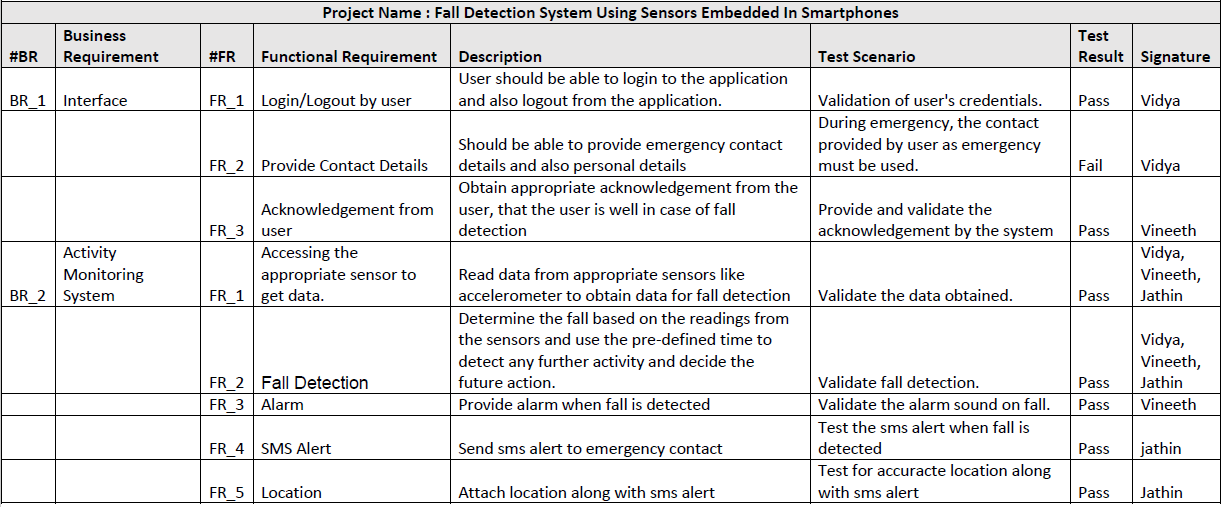
\includegraphics[width=9cm,height=4cm]{RTM_V2.PNG}}
\caption{Requirement Tracebility Matrix}
\label{fig2}
\end{figure}

\section{Project Estimation}
Function Point Analysis and COCOMO model\cite{b4} helps to predict the development time and effort for the project. On analysis 1609.3 lines of code were estimated, considering the language factor for JAVA which is assumed to be 38 the following figures were estimated,
 \begin{itemize}
\item Source Lines of Code: SLOC = 1609.3
\item Programmer Productivity:PM = 3.95530 person/month
\item Development time: DEV = 4.2156 months
\end{itemize}

\section{Responsibilities of all team members}
Figure.~\ref{resourceUtilization} shows the responsibility of all team members. The whole team is involved in major activities such as requirement analysis, design, and Implementation. The activities such as project vision, cost estimation, and testing are handled individually.
\begin{figure}
\centerline{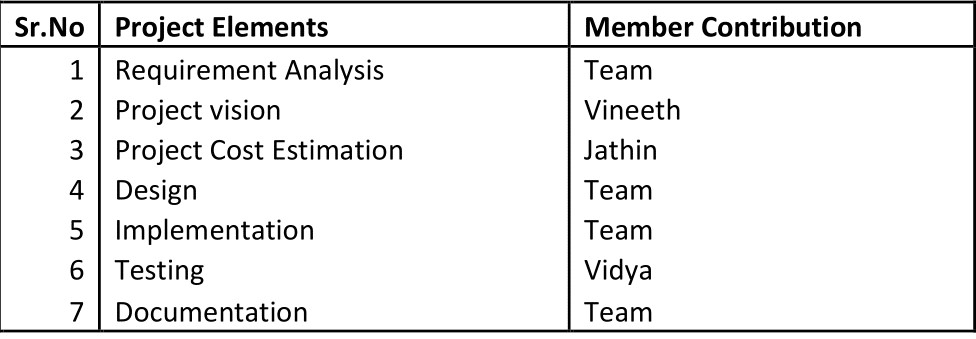
\includegraphics[width=7cm,height=2.5cm]{resourceUtilization.png}}
\caption{Resource Utilization}
\label{resourceUtilization}
\end{figure}

\section{Security}
\begin{itemize}
\item Privacy of user information. Example location, login data.
\item Confidentiality of the data collected from the sensor.
\item Requesting access permission to monitor the activity and device features.
\item User authentication for accessing the app and data. 
\item Sensor data can not be accessed from outside the Smartphone.
\end{itemize}

\section{Reliability}
\begin{itemize}
\item Accurate detection of fall based on sensor readings.
\item The data collected from the sensor must be reliable for any further use.
\item Activity monitored must be accurate.
\item Capability to handle a large amount of data and perform as intended.
\item State of the application is uninterrupted by the external interruption.
\end{itemize}

\section{Project Design}
Considering the above-mentioned requirements we have hashed out the following design for our project.

\subsection{Use Case Diagram}
Figure.~\ref{usecase} shows the interaction of the application with the user. Since the application detects fall based on sensor reading and activity tracking, we have kept the user interaction to a minimum. User logins to the application and provides the emergency details. Apart from this, the main feature would be checking the well being of the user in case of fall detected, in the form of an acknowledgment from the user.

\begin{figure}
\centerline{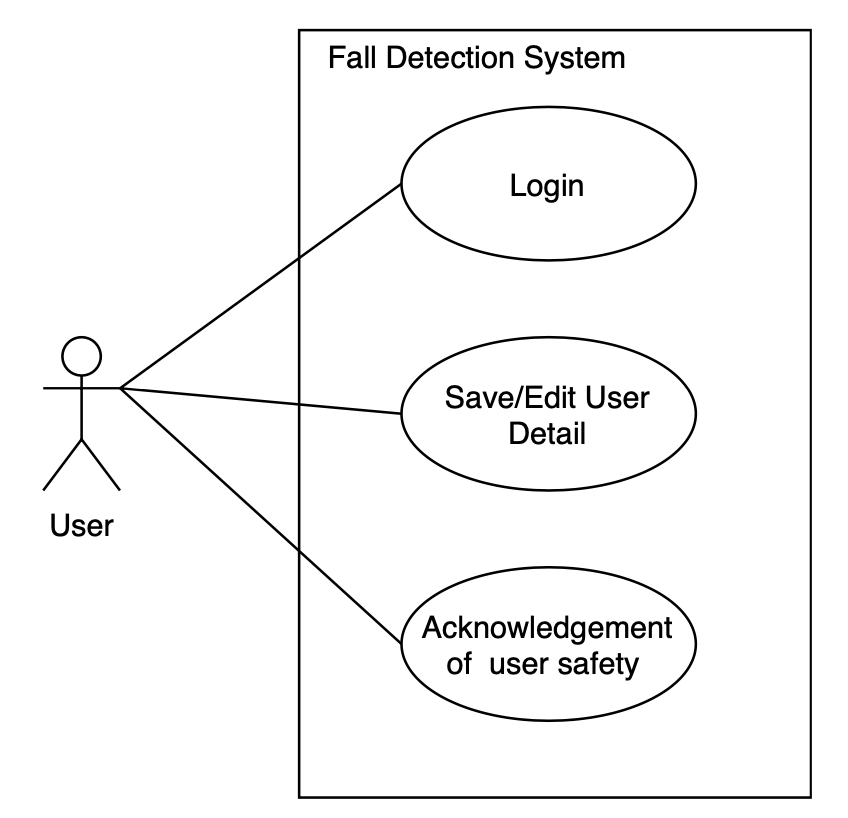
\includegraphics[width=4cm, height=4cm]{usecase.png}}
\caption{Use case diagram}
\label{usecase}
\end{figure}

\begin{figure}
\centerline{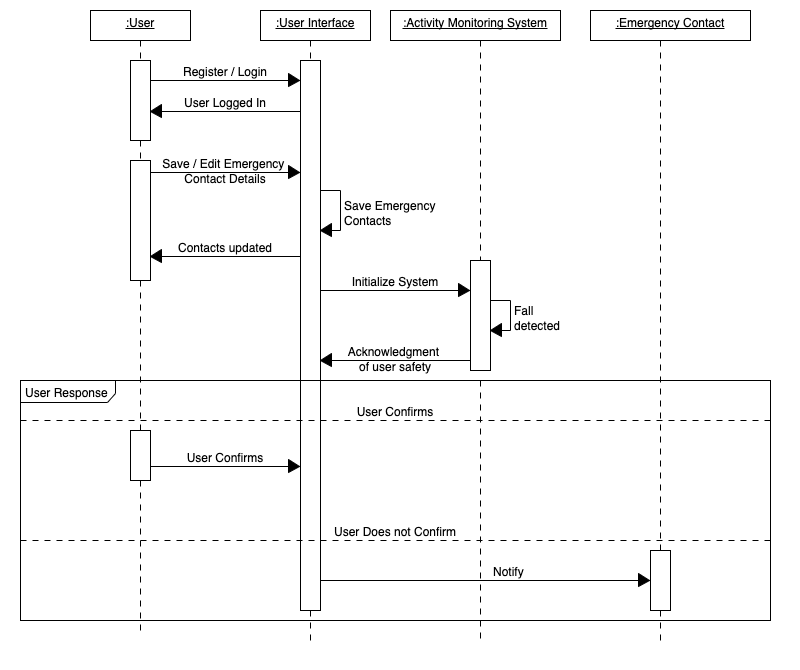
\includegraphics[width=8.25cm, height=7.25cm]{sequenceDiagram.PNG}}
\caption{Sequence Diagram}
\label{sequenceDiagram}
\end{figure} 

\subsection{Sequence Diagram} 
The sequence diagram (Figure.~\ref{sequenceDiagram}) explains the object interaction in a time sequence. User, UI, Activity Monitoring System, Sensors, and Emergency contact are involved in the interaction. The user initiates the Activity Monitoring System by logging into the application and providing emergency contact details. Once initiated, the system reads the gyroscope and accelerometer sensor data to tracks the activity by calculating the total sum vector, angular velocity, and tilt value. Tilt is estimated by a complementary filter using gyroscope and accelerometer values which detects fall, in case of any the system requests the user for an acknowledgment that he can carry on. Here there are two possible cases. Case 1: If the user confirms that he is well and that it is a false alarm then the system will not trigger alert to the emergency contact. Case 2: If the user does not acknowledge, then the system considers the user has fallen down and needs assistant and contacts the emergency contact.

\subsection{Class Diagram}
Figure.~\ref{classDiagram} explains the project architecture, explaining the class files and the functions involved in the project.

\begin{figure}
\centerline{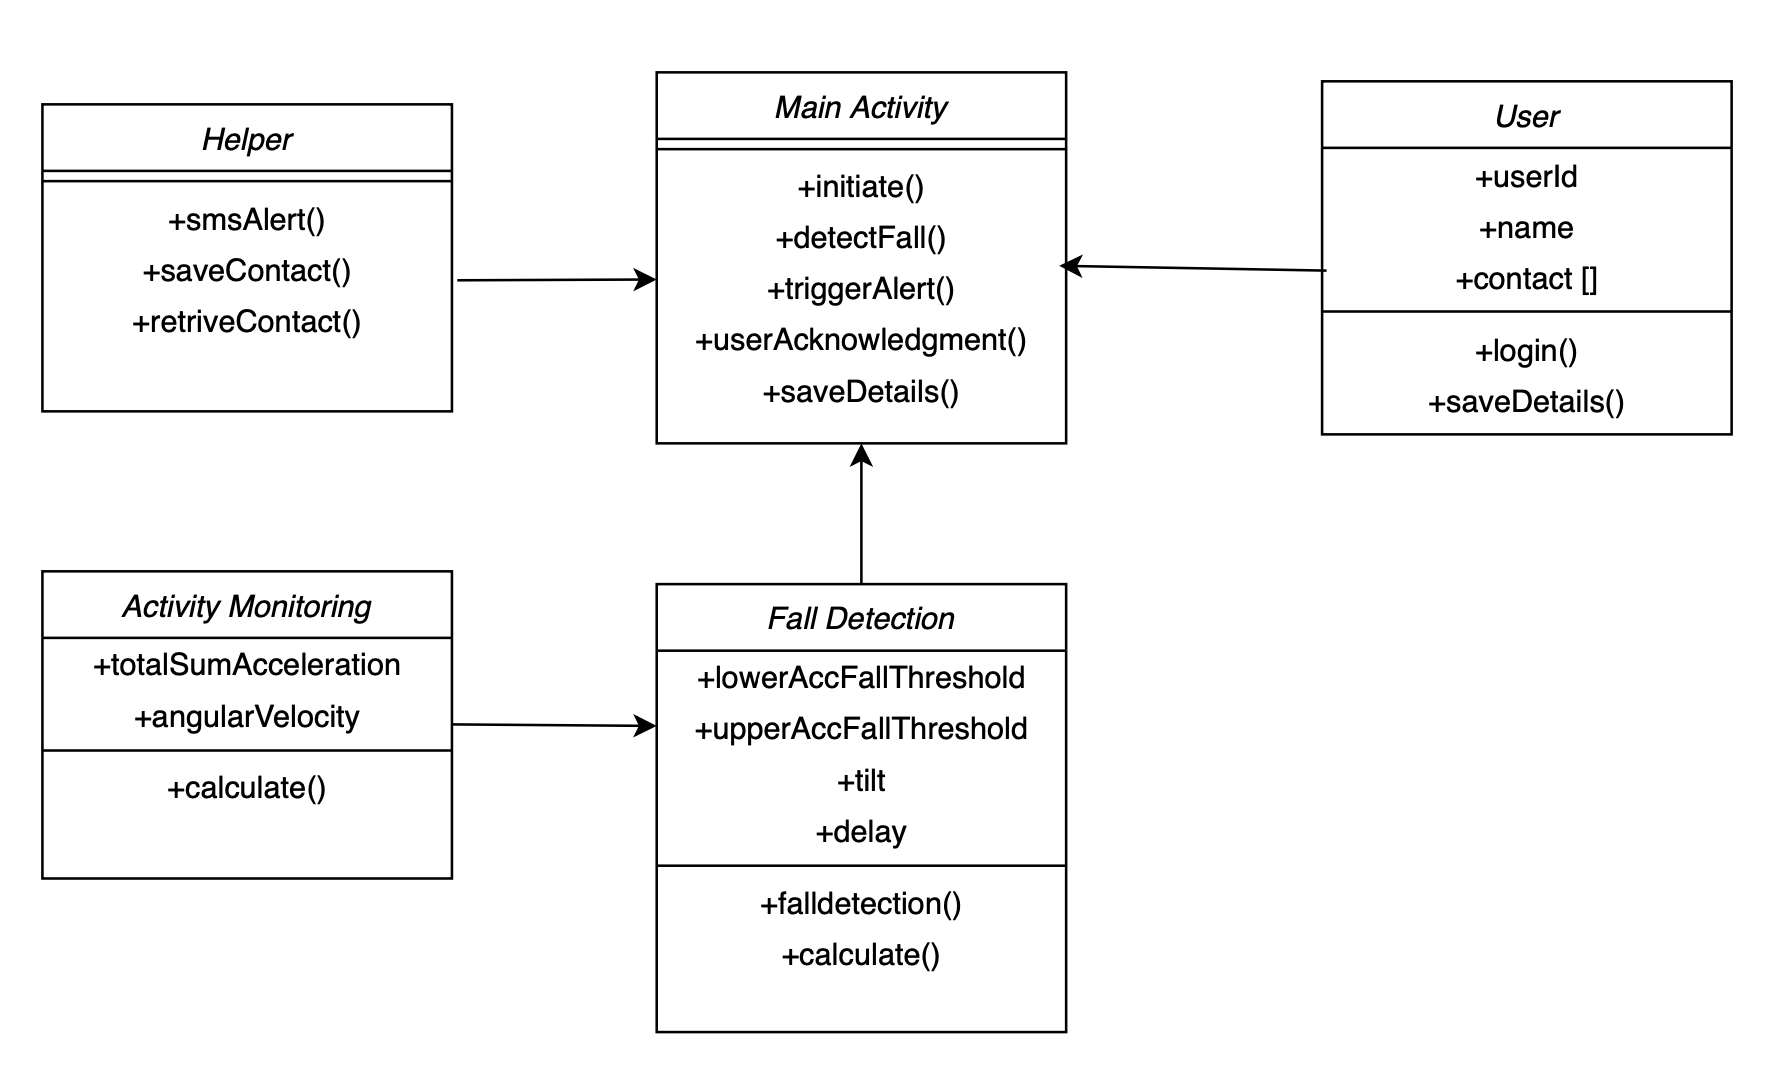
\includegraphics[width=8cm, height=6cm]{classDiagram.png}}
\caption{Class Diagram}
\label{classDiagram}
\end{figure}

\section{Development Environment}
Considering the android as our development environment due to usage of android devices in the team.\\
By using the Android sensor framework, accessing the available sensors and acquire the raw sensor data is easy. Android provides a dedicated hardware package for accessing the embedded sensors. It includes a sensor framework that provides certain classes and interfaces like, SensorManager, Sensor, SensorEvent, SensorEventListner to perform a variety of sensor-related tasks \cite{b1}. The following list specifies the hardware and software used in our project.
\begin{itemize}
    \item Smartphone: Google Pixel
    \item Operating System: Android
    \item IDE: Android Studio
    \item Version Control: GitHub
\end{itemize}

\subsection{Sensors Used}
There are various number of sensors that the android platform provides, the application uses the following sensors,\\
Accelerometer: In the device like smartphones the accelerometer measures the acceleration that is applied to a device on all three axes (x, y, and z), including the force of gravity. Using this we track the movement of the phone, and also to track the orientation and acceleration force on the device. \\
Gyroscope: The gyroscope sensor is a device that can measure the angular velocity of an object. They are more stable than the accelerometer.  The Coriolis force concept is used in the Gyroscope sensors to measure the device's rate of rotation around each of the three physical axes (x, y, and z). \\
Magnetometer: The Magnetometer sensor reads the strength of the magnetic field around the device. The sensors measure the physical position of a device based on the ambient magnetic field, the sensor produces a voltage which is proportional to the strength and polarity of the magnetic field along the each of the 3 axes.

\section{Fall Detection Algorithm}
 Based on previous studies \cite{b9} which involved the simulation of fall on 6 young healthy people ranged in age from 30 to 39 years (35.2 $\pm$ 2.2 years) old, with the body mass of 59 to 76 kgs (75.2 $\pm$ 2.2 kgs) and the height of the user should be around 1.68 to 1.76 m (1.75 $\pm$ 2.2 m), for 8 different types of simulated-falls. We are concentrating on only two types of falls forward fall and the backward fall. Each type of fall can be detected using the threshold-based algorithm. Threshold-based algorithms are preferred as these algorithms require low computational cost and lower complexity. This fall detection algorithm as depicted in (Figure.~\ref{fig:fallDetectAlgo}), defines several parameters depending on the accelerometer and gyroscope outputs, and a decision is made using the threshold values for these parameters. The parameters used in the algorithm are The total sum acceleration vector \(SV\) and The angular velocity \(omega\) and the angle or the actual orientation \(theta\). The total sum acceleration vector is calculated by,
\begin{equation}
 SV = \sqrt{(A_x)^2 + (A_y)^2 + (A_z)^2}\label{eq:1}
 \end{equation}
 
where \(A_x\), \(A_y\) and \(A_z\) are the reading from the accelerometer along the x, y and z axes. The angular velocity \(\omega\) is calculated by, 
\begin{equation}
\omega = \sqrt{(\omega_x)^2 + (\omega_y)^2 + (\omega_z)^2}\label{eq:2}
\end{equation}
where \(\omega_x\), \(\omega_y\) and \(\omega_z\) are readings from the gyroscope along the x, y and z axes.\\
The  orientation is calculated by integrating the angular velocity over time,

\begin{equation}
\theta = \int_{t1}^{t2} \omega dt\label{eq:3}
\end{equation}

where t1 is the previous sensor output and t2 is the current sensor output.
When the user falls, the total sum vector, angular velocity and tilt are calculated and compared against the thresholds values FT1, FT2 and FT3 respectively which are explained in the bellow section.
\begin{itemize}
    \item FT1 (upper acceleration threshold): This corresponds to value after the user hits the floor, which is a large pike depending on how hard the user has fallen to the ground. FT1 is set to 2.1g. The figure \ref{FT1} shows the change in acceleration occurred when fall is detected as compared to normal activities like walking.
\begin{figure}
\centerline{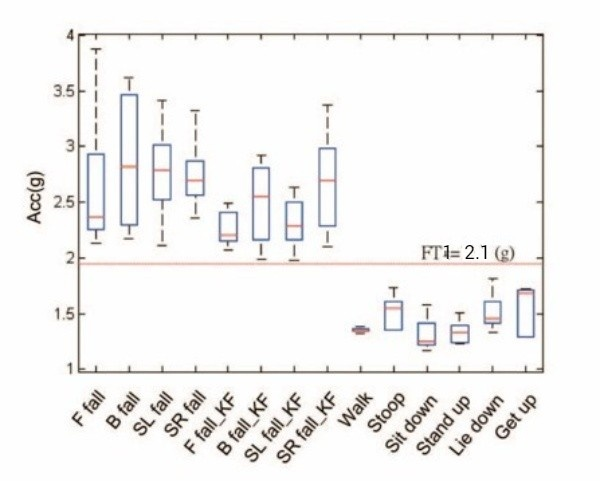
\includegraphics[width=7cm, height=5cm]{FT1 V2.png}}
\caption{Lower peak values FT1 for 8 types of simulated-fall and 6 types of different activities of daily living.}
\label{FT1}
\end{figure}
    \item FT2 (Angular velocity): Corresponds to the angular velocity when the user falls on the floor, FT2 is set to 3.1 rad/sec as per the reference\cite{b8},  which proves that the user has actually fallen on the ground and avoids false detection such as if the user sits on the sofa. Figure \ref{FT2} shows the changes in the gyro value when the fall detected for the activities like sit down, lie down and various other activities.

\begin{figure}
\centerline{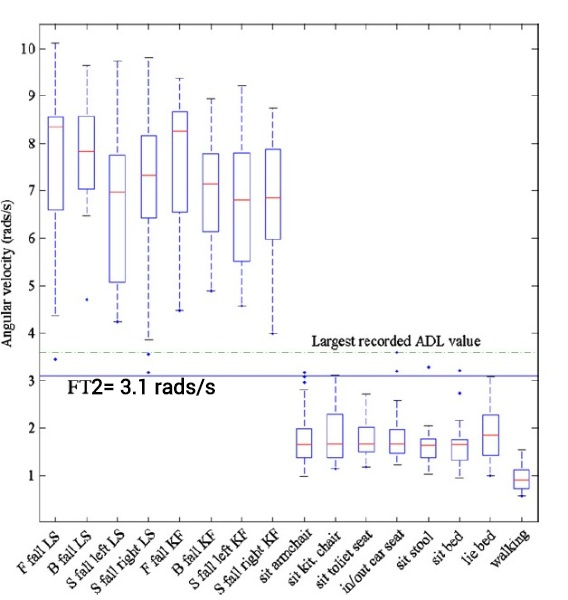
\includegraphics[width=6cm, height=5cm]{FT2 updated.png}}
\caption{Boxplot of peak values for falls and ADL. The horizontal axis crosses at 3.1 rad/s which is the FT2 value.\cite{b8}}
\label{FT2}
\end{figure}    

 \item FT3 (Theta): When the user falls, it detects the lying position by checking if the body angle exceeds the threshold value FT3. Taking reference from the paper \cite{b7} this is set to 60°.


\end{itemize}
When the user falls, the total sum vector increases above FT1 (2.1g), the angular velocity increases above FT2 (3.1 rads/s) and tilt exceeds FT3 (60 deg). Overall, if the application has detected a fall, but the user was not affected because of the fall, to avoid sending an alert message in this case the application brings up a notification for the user to acknowledge that the user has not fallen. If the user acknowledges that he has not fallen, the emergency contact is not notified, else an SMS is sent to the emergency contact which comprises of location.

 
\begin{figure}
\centerline{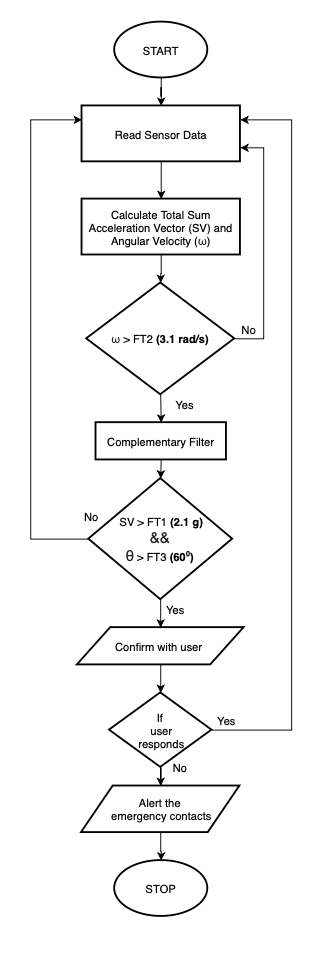
\includegraphics[width=4cm, height=11cm]{Flowchart_v3.1.png}}
\caption{Fall Detection Algorithm Flowchart}
\label{fig:fallDetectAlgo}
\end{figure}

\section{Measuring Errors and Sensor Fusion}
Errors obtained while using the sensors will add to the final output, thereby making the sensor readings inaccurate. Various errors contribute to the inaccuracy of a sensor. Accelerometer, magnetometer, and gyroscope would produce distinct errors. Accelerometers and magnetometers tend to be noisy. They produce small fluctuations in their readings that are picked up from the surrounding environment and vibrations. Whereas the gyroscope is more accurate in the short interval but would produce gyro drift over time. Gyro drift would be drifting of gyroscope towards an axis due to the small errors introduced in each step of integration over time, resulting in one slow constant orientation.
To eliminate errors the concept of sensor fusion is used, here the data from different sensors are combined to eliminate the errors and produce one final filtered output. There are various methods to carry out the filtering procedure, we have adopted the complementary filter method where the final output would be much smoother as shown in figure \ref{sensorFusion}.

\subsection{Complementary Filter}
The complementary filter as illustrated in Figure. \ref{fig:ComplimentaryFilterPrinciple} uses both accelerometer and gyroscope to estimate tilt ($\theta$). The data from the gyroscope is used for the short term, as the data is precise and not susceptible to external forces, but for the long term, the filter depends on the data from the accelerometer to prevent gyro drift. In the application to calculate tilt ($\theta$), when the application is initialized, the gyroscope data is not processed until the orientation angles are available from the accelerometer and magnetometer. This angle calculated from the accelerometer and the magnetometer is used as an initial orientation for the gyroscope data. After this, the complementary filter uses the data from the accelerometer and performs low-pass filtering on low-frequency tilt estimation, while it uses the gyroscope data directly integrated to the high pass filter and performs a biased high-frequency tilt estimation. Then the two tilt are combined which gives an all-pass estimation of the tilt. The mathematical model for the complementary filter can be represented as,
\begin{equation}
\theta\textsubscript{Angle} = \alpha * (\theta\textsubscript{Angle} + \omega\textsubscript{Gyro} * dt) + (1 - \alpha) * a\textsubscript{Acc} \label{eq:4}
\end{equation}
where $\theta\textsubscript{Angle}$ is the tilt estimation, $\alpha$ is the filter coefficient, $\omega\textsubscript{Gyro}$ represents the gyroscope output, and $a\textsubscript{Acc}$ is the accelerometer output. The value of 0.98 has been considered for the filter coefficient ($\alpha$) with a sampling rate of 33Hz for a time period of 30ms.

\begin{figure}
\centerline{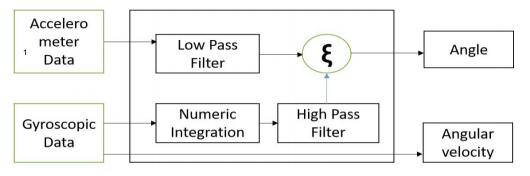
\includegraphics[width=9cm, height=3cm]{ComplimentaryFilterAlgorithm.png}}
\caption{Complimentary Filter Principle\cite{b10}}
\label{fig:ComplimentaryFilterPrinciple}
\end{figure}

\begin{figure}
\centerline{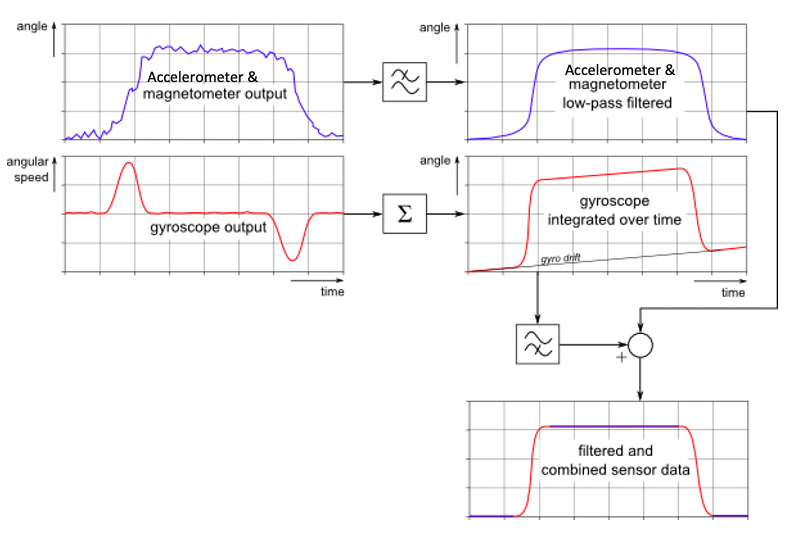
\includegraphics[width=9cm, height=6cm]{sensorFusion.png}}
\caption{Data filtering by sensor fusion using complementary filter  \cite{b11}}
\label{sensorFusion}
\end{figure}


\section{Results}
\subsection{Testing}
The application was tested by simulating the MobiFall dataset\cite{b12}. This dataset was developed by the Biomedical Informatics & eHealth Laboratory of the Technological Educational Institute of Crete. The second release of the MobiFall dataset contains datasets from 24 volunteers - 17 males and 7 females, 22 years to 47 years old who weight between 50 to 103 kgs. The datasets were collected via a smartphone which was located in a trouser pocket freely chosen by the subject in any random orientation. 9 participants performed both falls and Activities of Daily Living (ADL), while 15 participants performed only falls. The datasets of two types of falls (Forward and Backward Falls) and 9 types of ADL (common everyday activities like walking, standing, jumping, and jogging) were considered for testing. The datasets provide accelerometer and gyroscope data along all the three axes with the timestamp for each sample.
\subsection{Test Results}
For the above-mentioned dataset, the sensitivity that is the proportion of falls that are correctly detected and specificity that is the proportion of non-fall events that are correctly detected \cite{b14} are calculated based on the data collected as shown in Figure 
\ref{result}. The sensitivity came out to be 0.7708 and the specificity was 0.7777. 

\section{Conclusion And Future work}
Considering the test results, the simple algorithm based on the thresholds, detected the majority of the falls and correctly ignored the daily activities. To improve the results of the application the threshold must be varied considering a higher number of falls and ADL and defining more accurate thresholds. As the application is developed on a smartphone, which provides various advantages such as providing an alarm in case of fall detected and if the user is actually in danger sending a message along with the current location to the emergency contact. Future work would be to enhance the application interface for easier interaction and conducting the test on wider subject groups and more considering various other fall types.

\begin{figure}
\centerline{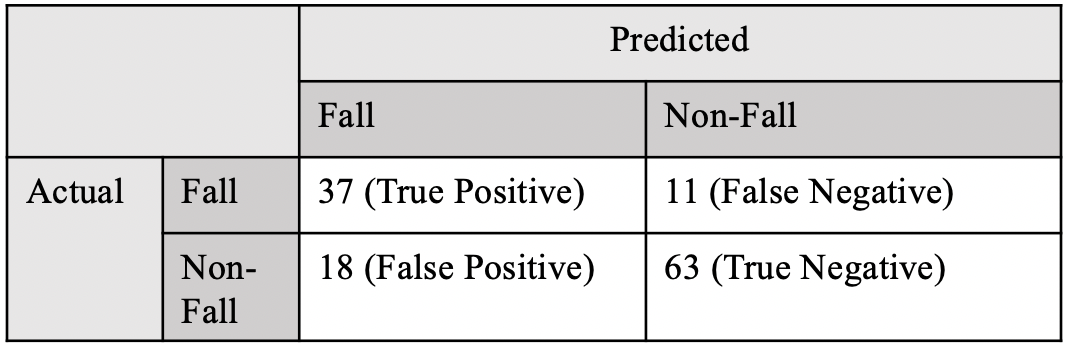
\includegraphics[width=8cm, height=2.5cm]{results.png}}
\caption{Test Results for the dataset}
\label{result}
\end{figure}

\begin{thebibliography}{00}
\bibitem{b1} Sensors: https://developer.android.com/guide/topics/sensors Accessed: 09.06.2020
\bibitem{b2} Gyroscope:
https://ef.engr.utk.edu/hyperphysics/hbase/gyr.html Accessed: 09.06.2020
\bibitem{b3} Live Science: https://www.livescience.com/40102-accelerometers.html Accessed: 09.06.2020
\bibitem{b4} Cost Estimation, Padmaja,  http://people.cs.ksu.edu/~padmaja/Project/CostEstimate.html,  Accessed: 09.06.2020
\bibitem{b5}E. Thammasat and J. Chaicharn, "A simply fall-detection algorithm using accelerometers on a smartphone," The 5th 2012 Biomedical Engineering International Conference, Ubon Ratchathani, 2012, pp. 1-4, doi: 10.1109/BMEiCon.2012.6465471.
\bibitem{b6}F. Sposaro and G. Tyson, "iFall: An android application for fall monitoring and response," 2009 Annual International Conference of the IEEE Engineering in Medicine and Biology Society, Minneapolis, MN, 2009, pp. 6119-6122, doi: 10.1109/IEMBS.2009.5334912.
\bibitem{b7}S. Abdelhedi, R. Bourguiba, J. Mouine and M. Baklouti, "Development of a two-threshold-based fall detection algorithm for elderly health monitoring," 2016 IEEE Tenth International Conference on Research Challenges in Information Science (RCIS), Grenoble, 2016, pp. 1-5, doi: 10.1109/RCIS.2016.7549315.
\bibitem{b8}Bourke, Alan & ÓLaighin, Gearóid. (2008). A threshold-based fall-detection algorithm using a bi-axial gyroscope sensor. Medical engineering & physics. 30. 84-90. 10.1016/j.medengphy.2006.12.001.
\bibitem{b9}H. W. Guo, Y. T. Hsieh, Y. S. Huang, J. C. Chien, K. Haraikawa and J. S. Shieh, "A threshold-based algorithm of fall detection using a wearable device with tri-axial accelerometer and gyroscope," 2015 International Conference on Intelligent Informatics and Biomedical Sciences (ICIIBMS), Okinawa, 2015, pp. 54-57, doi: 10.1109/ICIIBMS.2015.7439470.
\bibitem{b10}Islam,Tariqul  and Islam,Md. Saiful  and Shajid-Ul-Mahmud,Md.  and Hossam-E-Haider,Md, Comparison of complementary and Kalman filter based data fusion for attitude heading reference system, AIP Conference Proceedings, Vol. 1919, Number 1, doi:10.1063/1.5018520, 2017.
\bibitem{b11} Android Sensor Fusion Tutorial, Paul Lawitzki http://plaw.info/articles/sensorfusion/ Accessed: 08.07.2020
\bibitem{b12}G. Vavoulas, M. Pediaditis, E. G. Spanakis and M. Tsiknakis, "The MobiFall dataset: An initial evaluation of fall detection algorithms using smartphones," 13th IEEE International Conference on BioInformatics and BioEngineering, Chania, 2013, pp. 1-4, doi: 10.1109/BIBE.2013.6701629.
\bibitem{b13}G. Vavoulas, M. Pediaditis, C. Chatzaki, E. G. Spanakis, M. Tsiknakis, The MobiFall Dataset: Fall Detection and Classification with a Smartphone, invited publication for the International Journal of Monitoring and Surveillance Technologies Research, pp 44-56, 2014, DOI:10.4018/ijmstr.2014010103.
\bibitem{b14} Broadley, R.W.; Klenk, J.; Thies, S.B.; Kenney, L.P.J.; Granat, M.H. Methods for the Real-World Evaluation of Fall Detection Technology: A Scoping Review. Sensors 2018, 18, 2060.
\end{thebibliography}
\vspace{12pt}

\end{document}
